\documentclass[a4paper,12pt]{report} % добавить leqno в [] для нумерации слева

%%% Работа с русским языком
\usepackage{cmap}					% поиск в PDF
\usepackage{mathtext} 				% русские буквы в формулах
\usepackage[T2A]{fontenc}			% кодировка
\usepackage[utf8]{inputenc}			% кодировка исходного текста
\usepackage[english,russian]{babel}	% локализация и переносы

%%% Дополнительная работа с математикой
\usepackage{amsmath,amsfonts,amssymb,amsthm,mathtools} % AMS
\usepackage{icomma} % "Умная" запятая: $0,2$ --- число, $0, 2$ --- перечисление

%% Номера формул
\mathtoolsset{showonlyrefs=true} % Показывать номера только у тех формул, на которые есть \eqref{} в тексте.

%% Шрифты
\usepackage{euscript}	 % Шрифт Евклид
\usepackage{mathrsfs} % Красивый матшрифт

%% Свои команды
\DeclareMathOperator{\sgn}{\mathop{sgn}}

%\setlength\parindent{0ex}
%\setlength\parskip{0.3cm}

%%% Заголовок
\author{Волков Павел А-14-19}
\title{Типовой расчет №3 по численным методам Вариант 3}
\date{\today}

\usepackage{graphicx}

\begin{document} % конец преамбулы, начало документа

\maketitle

\newpage
\section*{Задание}
Найти корень нелинейного уравнения из задачи 2 методом простой итерации. Для этого преобразовать уравнение $f(x) = 0$ к виду, удобному для итераций и проверить выполнение условий сходимости. В качестве отрезка локализации взять отрезок, полученный методом бисекции при решении задачи 2. Найти корень методом простой итерации с точностью $\varepsilon = 0.0001$

\[
	f(x) = x^2 - 3x - \frac{1}{x + 1}
\]
\section*{Решение}

\subsection*{Выбор итерационной функции}

Выберем итерационную функцию и проверим условие сходимости на отрезке локализации $[2, 4]$.

На графике представлены производные 3-х итерационных функций:
\begin{gather*}
	\varphi_1 (x) = \frac{1}{3}(x^2 - \frac{1}{x+1}) \\
	\varphi_2 (x) =  \sqrt{3x + \frac{1}{x+1}}\\
	\varphi_3(x) = \frac{1}{x^2 - 3x} - 1
\end{gather*}
\noindent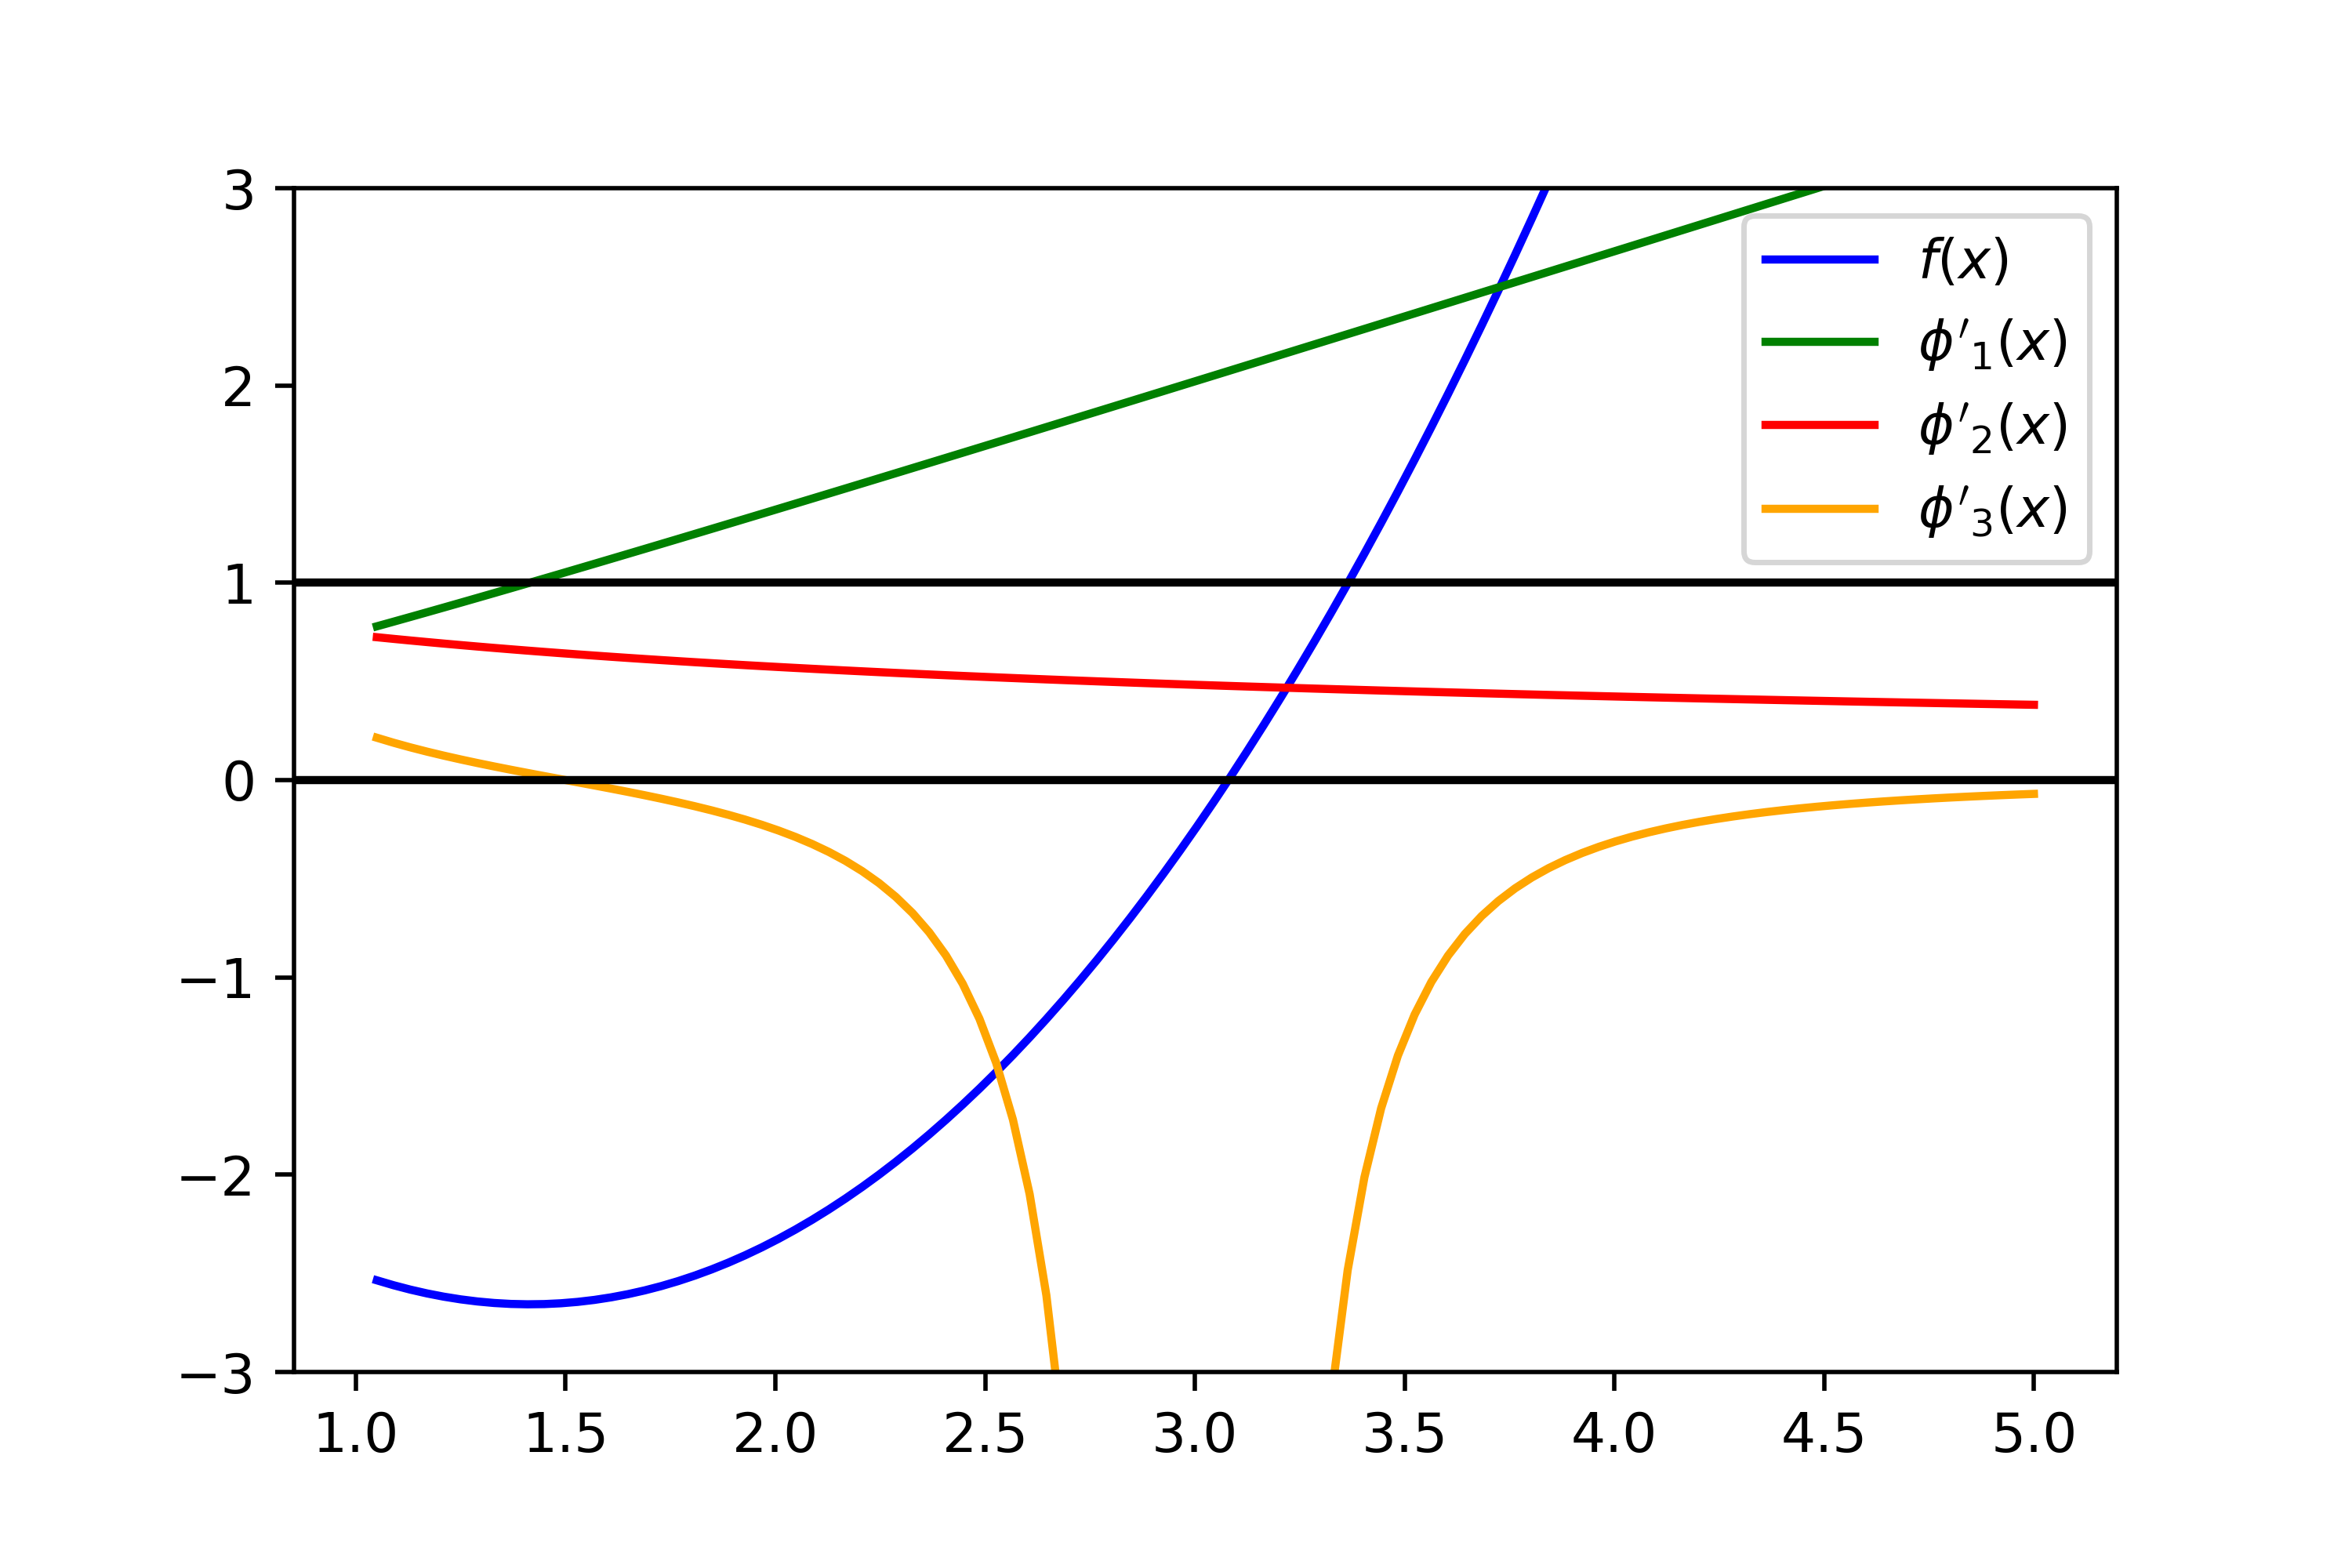
\includegraphics[height=8cm]{rout_calc_3.png}

\newpage
Из графика следует, что условию сходимости удовлетворяет вторая итерационная функция, причем:
\[
	max(|\varphi'_2(x)|)_{[2, 4]} = |\varphi'_2(2)| \leq 0.6 = q
\]

\subsection*{Применение метода}

Запишем расчетную формулу метода простой итерации:
\[
	x^{(k+1)} = \sqrt{3x^{(k)} + \frac{1}{x^{(k)} + 1}}
\]

\noindent В качестве начального приближения возьмем середину отрезка $x^{(0)} = 3$:

\begin{tabular}{ | c | c | c |}
	\hline
	$k$ & $x^{(k)}$ & $|x^{(k)} - x^{(k-1)}|$ \\ \hline
	0 & 3 & -  \\ \hline
	1 & 3.0413812651491097 & 0.041381  \\ \hline
	2 & 3.0613042888283317 & 0.019923  \\ \hline
	3 & 3.0708531687726475 & 0.009549  \\ \hline
	4 & 3.075420013298832 & 0.004567  \\ \hline
	5 & 3.0776019109160693 & 0.002182  \\ \hline
	6 & 3.078643843839416 & 0.001042  \\ \hline
	7 & 3.079141287154193 & 0.000497  \\ \hline
	8 & 3.0793787517998505 & 0.000237  \\ \hline
	9 & 3.0794921043204835 & 0.000113  \\ \hline
	10 & 3.0795462111839926 & 0.000054  \\ \hline
\end{tabular}

Ответ: $\overline{x} = x^{(10)} \pm \varepsilon = 3.0795 \pm 0.0001$

\end{document}